%%%%%%%%%%%%%%%%% your_thesis_eng.tex %%%%%%%%%%%%%%%%%
%
% This is the template file for ORM 2016 proceedings.
%
% Please, fill in following the directions below.
%
%%%%%%%%%%%%%%%%%%%%%%%%%%%%%%%%%%%%%%%%%%%%%%%%%%%%%%%

\Title[%
% Insert here the acknowledgements of grants and/or any other
% information you wish to appear as a footnote, or leave this
% field blank.
This research is supported by\ldots%
]
{%
% Insert your title here
Title of your thesis%
}
{%
% Insert the authors' names here
A.I.~Pyanykh%
}
{%
% Insert your institution here
Moscow State University%
}
{%
% Insert your city here
Moscow%
}
{%
% Insert your country here
Russia%
}

% Insert your thesis here.
% The entire submission should not exceed 3 pages if you plan a publication in conference proceedings.
%
% ATTENTION: Using 'thebibliography' environment is not allowed.
% Use 'references_eng' environment below to format the list of references.
% Please note that the latter environment does not provide automatic
% citation facilities. Cite manually using square brackets,
% e.g., [1], [2, 3], [4--6].
%
Your thesis. This work relies on the results in [1], and is an extension of the development in [2, 3].

% Insert your figure, if needed.
\begin{figure}[!h]
  \centering
  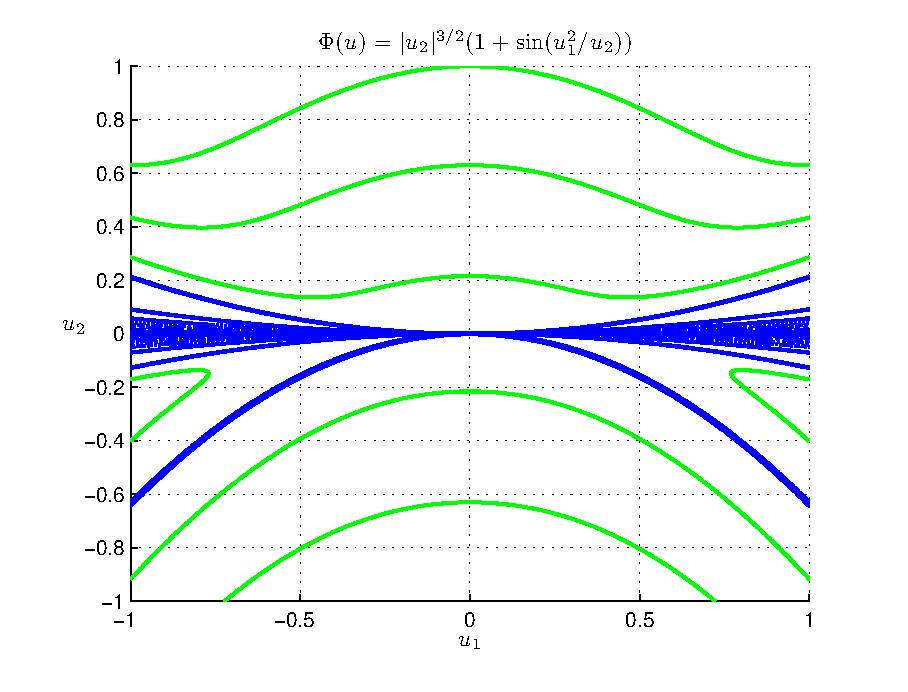
\includegraphics[width=0.7\maxpicturewidth]{your_figure.eps}
  \center{Fig.~1. Your caption.}
\end{figure}

\begin{references_eng}
% Insert your list of references here. The order of items in the list must
% agree with the order of their appearance in the text of your thesis.
% Use the '\url' command for citing url-s: e.g., \url{http://http://www.mathopt.org/}.

  \item % Reference No. 1
  Taylor~T.T. Article in a collection // Collection title. New York: Springer, 2012. P.~1--21.

  \item % Reference No. 2
  Smith~S.S. Book. New York: Springer, 2012.

  \item
  Baker~B.B. Journal article // Journal title. 2012. V.~1, \No ~1. P.~1--21.

% ...

\end{references_eng}

%%%%%%%%%%%%%%%%%%%%%%%%%%%%%%%%%%%%%%%%%%%%%%%%%%%%%%%

%%% Local Variables:
%%% mode: latex
%%% TeX-master: "main"
%%% End:
